% Template for PLoS
% Version 1.0 January 2009

\documentclass[10pt]{article}

% amsmath package, useful for mathematical formulas
\usepackage{amsmath}
% amssymb package, useful for mathematical symbols
\usepackage{amssymb}

% graphicx package, useful for including eps and pdf graphics
% include graphics with the command \includegraphics
\usepackage{graphicx}

% cite package, to clean up citations in the main text. Do not remove.
\usepackage{cite}

\usepackage{color} 

% Use doublespacing - comment out for single spacing
%\usepackage{setspace} 
%\doublespacing


% Text layout
\topmargin 0.0cm
\oddsidemargin 0.5cm
\evensidemargin 0.5cm
\textwidth 16cm 
\textheight 21cm

% Bold the 'Figure #' in the caption and separate it with a period
% Captions will be left justified
\usepackage[labelfont=bf,labelsep=period,justification=raggedright]{caption}

% Use the PLoS provided bibtex style
\bibliographystyle{plos2009}

% Remove brackets from numbering in List of References
\makeatletter
\renewcommand{\@biblabel}[1]{\quad#1.}
\makeatother


% Leave date blank
\date{}

\pagestyle{myheadings}
%% ** EDIT HERE **


%% ** EDIT HERE **
%% PLEASE INCLUDE ALL MACROS BELOW

\newcommand{\Kcomment}[1]{{\color{blue}{[KJ: #1]}}}
\newcommand{\Acomment}[1]{{\color{red}{[AE: #1]}}}

\DeclareMathOperator{\Tr}{tr}
\newcommand{\mcond}{\,\middle\vert\,}
\newcommand{\cond}{\,\vert\,}
\newcommand{\loss}[1]{\mathcal L\left(#1\right)} 
\newcommand{\T}{{\sf T}}
\newcommand{\E}[2][]{\mathbb E_{#1}\left[ #2\right]}    % expected value
\newcommand{\TODO}[1]{\emph{\small\color{blue}$\langle\langle$#1$\rangle\rangle$}}
\newcommand*\dif{\mathop{}\,d}
\DeclareMathOperator*{\argmin}{arg\,min}
\DeclareMathOperator{\rank}{rank}

%% END MACROS SECTION

\begin{document}
% Title must be 150 characters or less
\begin{flushleft}
{\Large
Improved estimation of neural correlations suggests detailed interactions in visual cortex
}
% Insert Author names, affiliations and corresponding author email.
\\
Dimitri Yatsenko,$^{1,\ast}$, 
Kre\v{s}imir Josi\'{c}$^{2}$,
Alexander S.~Ecker$^{1,3,4}$,
Emmanouil Froudarakis$^{1}$,
R.~James Cotton$^{1}$,
Andreas S.~Tolias$^{1,5}$
\\
\bf{1} Department of Neuroscience, Baylor College of Medicine, Houston, TX, USA
\\
\bf{2} Department of Mathematics and Department of Biology and Biochemistry, University of Houston, Houston, TX, USA
\\
\bf{3}  Werner Reichardt Center for Integrative Neuroscience and Institute for Theoretical Physics, University of T\"ubingen, Germany
\\
\bf{4} Bernstein Center for Computational Neuroscience, T\"ubingen, Germany
\\
\bf{5} Department of Computational and Applied Mathematics, Rice University, Houston, TX, USA

$\ast$ E-mail: yatsenko@cns.bcm.edu
\end{flushleft}

\section*{Abstract}
% Please keep the abstract between 250 and 300 words
Correlations between the spiking activity of pairs of neurons are among the most familiar descriptive statistics of neural activity.
Multineuronal recordings provide richer information than the equivalent number of neuron pairs.
For example, the full covariance  matrix reveals correlated activity across the entire population as well as partial correlations between pairs.
Estimation of covariance matrices can be improved by regularization, \emph{i.e.}\;by imposing some kind of structure.
Optimal regularization must be determined empirically since its effect depends on how closely the imposed structure matches the underlying regularities.
For example, we can use low-rank parameterizations of the covariance matrix to account for common fluctuations across the recorded population.
Conversely, if correlations are strongly influenced by a small fraction of pairwise linear associations between the observed neurons, we can impose sparsity on the inverse covariance matrix.

We can also use a \lq sparse+low rank\rq inverse covariance representation to account for both common fluctuations and pairwise interactions.  
To select the optimal structure of neural correlations in a local neural circuit, we compared the performance of several covariance estimators on the activity of 100--300 neurons in mouse visual cortex: sample covariance, covariance shrinkage, factor analysis, sparse inverse covariance, and sparse+low-rank inverse covariance. We inferred instantaneous firing rates in 200 ms bins from the somatic calcium signals acquired with fast 3D random-access two-photon microscopy.  Each covariance estimator was optimized and evaluated by cross-validation. As expected, covariance shrinkage reliably outperformed the sample covariance estimate. In turn, factor analysis-based estimates significantly outperformed covariance shrinkage. Yet sparse inverse covariance with or without an additional low-rank component significantly outperformed both factor analysis and shrinkage estimators. The superior performance of the sparse inverse covariance estimator suggests the relative importance of detailed network interactions over common diffuse input in the circuit we studied.

% Please keep the Author Summary between 150 and 200 words
% Use first person. PLoS ONE authors please skip this step. 
% Author Summary not valid for PLoS ONE submissions.   
\section*{Author Summary}
Covariance matrices of the activity of populations of neurons are useful descriptions of the functional organization of neural circuits with implications for stimulus coding and neural circuit architecture. 
Estimates of the covariance matrix can be dramatically improved by \emph{regularization}, \emph{i.e.}\;the biasing of the usual estimate toward one of several possible low-dimensional approximations, the \emph{target estimate}. However, the amount of improvement depends on how closely the selected approximation reflects the dominant interactions in the circuit. 
In simulation, we demonstrated that no regularized estimate was universally superior to others: each performed best when the target estimate was the closest match to the structure of the data generating process. 
We then evaluated covariance matrix estimates on the calcium activity recorded \emph{in vivo} from large populations of closely spaced neurons  in mouse primary visual cortex, after subtracting the average stimulus response.
Using cross-validation, we found that the best estimate was produced when the covariance matrix was approximated as that of a sparse Gaussian graphical models with a small number of latent units. 
Thanks to the paucity of their parameters, these optimally estimated covariance matrices also help interpretation of the covariance structure and allow relating the functional organization of the neural circuit to its cytoarchitecture.

\section*{Introduction}
Pearson correlations between the spiking activity of pairs of neurons, or simply \emph{neural correlations}, are the most familiar descriptive statistics of neural population activity \cite{Averbeck:2006,Zohary:1994,Kohn:2005,Bair:2001,Renart:2010}.  
For example, \emph{noise correlations}, \emph{i.e.}~the correlations of stimulus response variability between pairs of neurons, have been of particular interest.  
Noise correlations can have profound theoretical implications for stimulus coding \cite{Zohary:1994,Abbott:1999,Averbeck:2006,Berens:2011,Ecker:2011}, and have been interpreted to indicate detailed and specific functional organization. 
Such interpretation is supported by a series of discoveries of nontrivial relationships between neural correlations and other aspects of circuit organization such as the physical distance separating the neurons \cite{Smith:2008,Denman:2013}, their synaptic connectivity and stimulus tuning similarity \cite{Kohn:2005,Ko:2011}, cortical layer specificity \cite{Hansen:2012,Smith:2013}, cell-type specificity (?), progressive changes in development and in learning \cite{Golshani:2009}, changes due to sensory stimulation and global brain states \cite{Goard:2009,Kohn:2009,Ecker:2010,Renart:2010}, and others.

However, neural correlations do not come with ready or unambiguous mechanistic interpretations.
Theoretical and simulation studies have shown that neural correlations, rise at various temporal scales from combinations of multiple underlying mechanisms.
These include direct synaptic interactions, common or correlated inputs, shared sensory noise, chains of multiple synaptic connections, oscillations, top-down modulation, and background network activity \cite{Perkel:1967b,Shadlen:1998,Salinas:2001,Ostojic:2009,Rosenbaum:2011}.

Early studies of neural correlations were based on measurements from isolated pairs of neurons and their impact on coding was extrapolated to entire populations \cite{Shadlen:1998,Zohary:1994}.
Multineuronal recordings allow estimation of covariance matrices of large populations of neurons.
Such estimates provide more information than the equivalent number of pairwise correlations assessed in isolation.
Indeed, the correlation matrix is greater than the sum of its parts: it can be transformed into other representations that accentuate different aspects of the correlation structure and may suggest different mechanistic interpretations.
For example, the eigenvalue decomposition of the covariance matrix expresses shared correlated activity components across the population; common fluctuations of population activity may be accurately represented by just a few principal components but will affect all correlation coefficients.
In contrast, the off-diagonal elements of the inverse of the correlation matrix constitute scaled partial correlations between neuron pairs, which reflect their specific linear dependencies, after accounting for the activity of all the other recorded cells; a strong interaction between a pair of neurons may be expressed by a single partial correlation but its effects may propagate to multiple correlations and eigenvalues.
The inverse of the covariance matrix plays an important role in decoding schemes such as linear discriminant analysis, for example.
The mutliple  representations of the covariance matrix with their alternative interpretations add both complications and opportunities into the search for fundamental regularities in neural population activity. 

With large numbers of recorded cells, the usual estimations of the covariance matrix from finite recordings become ill-conditioned. Numerical instabilities arise because, as the amount of recorded data increases only linearly, the number of free coefficients to be estimated in any parameterization of the covariance matrix increases quadratically. 
For example, the large eigenvalues of large sample covariance matrices are biased upward while small eigenvalues are biased downward \cite{Ledoit:2004}. Similarly, the coefficients of the inverse covariance matrix require larger sample sizes to be estimated accurately from high-dimensional data than low-dimensional data.

With this study, we pursue two related goals: 
\begin{enumerate}
	\item Devise more efficient estimators of neural covariance matrices in recordings from large populations of neurons.
	\item Aid interpretation of neural covariance matrices.
\end{enumerate}

To select the best covariance matrix estimate for a specific neural circuit, we evaluate the performance of four estimators using different regularization schemes, each motivated by  a different hypothesis for the origin of neural correlations. \emph{Regularization} is the deliberate biasing the solution toward a simplified, low-dimensional (`sparse') \emph{target estimate} \cite{Schafer:2005,Bickel:2006}.
Regularized estimators allow reaching a favorable tradeoff between bias and variance in order to minimize the total error.

% Results and Discussion can be combined.
\section*{Results}

\subsection*{Covariance estimation}
We aim to estimate the true covariance matrix 
\begin{equation}\label{eq:true-covariance}
\Sigma = \E{(x-\mu)(x-\mu)^\T}
\end{equation}
where $\E{\cdot}$ denotes expectation; $x$ is the $p\times 1$ vector of real-valued instantaneous firing rates in bins of duration $\Delta t$. The vector of mean firing rates is $\mu = \E{x}$.  

The usual estimator of the covariance matrix is the \emph{sample covariance matrix} $C_0$ computed from the empirical sample of observations $x(1),\ldots,x(n)$ as
\begin{equation}
C_0 = \frac 1 \nu \sum\limits_{t=1}^n (x(t)-\mu)(x(t)-\mu)^\T, 
\end{equation}
where $\nu$ is the number of degrees of freedom per neuron in the sample ($\nu=n-1$ if observations are independent).  
The sample covariance matrix is unbiased, \emph{i.e.} $\E{C_0}-\Sigma=0$.
For finite sample sizes, however, $C_0$ is not as close to $\Sigma$ as a number of biased estimators.

Regularization is the deliberate biasing of the estimate toward a low-dimensional, less variable \emph{target estimate} to strike a favorable balance between bias and variability of the estimate \cite{Bickel:2006,Ledoit:2004}.  

The estimator whose target estimate most closely matches the true low-dimensional structure of the data is likely to outperform other estimators. This principle provides the logic of this study. 

We considered four regularized estimators based on distinct families of low-dimensional target estimates: `independent', `latent factors', `sparse interactions', and `sparse+latent' (Fig.~\ref{fig:02}\;row 1).  

In the first regularized estimator $C_{\sf diag}$, the target estimate is the diagonal matrix $D$ containing on its diagonal estimates of the variances.
The regularized estimate is obtained by linear \emph{shrinkage} of the unbiased estimate $C_0$ toward $D$ controlled by the scalar \emph{shrinkage intensity} parameter $\lambda \in [0, 1]$:
\begin{equation}
C_{\sf diag} = (1-\lambda) C_0 + \lambda D
\end{equation}
The diagonal target estimate expresses the idea of a lack of dependence (or of linear association) between the activity of observed neurons (Fig.~\ref{fig:02}\;A).  
If this assumption aptly describes recorded data, then strong shrinkage toward $D$ will add little bias while strongly reducing the variability of the estimate. Shrinkage allows for partial commitment to the low-dimensional representation.  

In the second regularized estimator $C_{\sf factor}$, the target estimate is the factor model $F =  L L^\T + \Psi$ with $d$ factors so that $L$ is the $p\times d$ matrix of \emph{factor loadings} and the diagonal matrix $\Psi$ contains the independent variances of each neuron.
Then the estimate is 
\begin{equation}
C_{\sf factor} = (1-\lambda) C_0 + \lambda F
\end{equation}
This estimator has two hyperparameters: the number of factors $d$ and shrinkage intensity $\lambda$. The target estimate $F$ expresses the assumption that correlated fluctuations in population activity are driven by a small number of latent factors that affect many cells while direct interactions between cells are insignificant (Fig.~\ref{fig:02}\;B).   

The third estimator $C_{\sf sparse}$ is based on the assumption that all correlations are the result of direct linear interactions between pairs of observed cells and that such interactions occur only between a fraction of such pairs (Fig.~\ref{fig:02}\;C).
This assumption is enforced by reducing to zero the majority of pairwise \emph{partial correlations} in the recorded population. 
While usual correlations are calculated from the marginal distribution without conditioning on all the other neurons, the partial correlation expresses the pairwise correlation conditioned on the activity of all the other cells.  
If cells only exert linear effects on each other and all neurons are recorded, partial correlations express the direct interactions between neurons. 
Therefore, this estimator is biased toward the assumption that correlations arise due to interactions between a subset of pairs of recorded neurons (Fig.~\ref{fig:03}C). When the partial correlation between a pair of neurons is zero, then the corresponding element of the inverse of the covariance matrix (often referred to as the \emph{precision matrix} or \emph{concentration matrix}) must be zero as well. Then the estimator is 
\begin{equation}
C_{\sf sparse} = S^{-1}
\end{equation}
where $\hat S$ is a sparse matrix with a large fraction of zeros in its off-diagonal elements. The estimate has one hyperparameter to regulate the sparsity (fraction of off-diagonal zeros) in $S$.

Finally, we consider the fourth estimator $C_{\sf sparse+lowrank}$, which provides for both common latent factors interacting with all recorded neurons and sparse interactions between the recorded neurons (Fig.~\ref{fig:02}\;D). This estimator has the form
\begin{equation}
C_{\sf sparse+latent} = (S - LL^\T)^{-1},
\end{equation}
where, as above, $S$ is a sparse matrix and $L$ is a $d\times p$ matrix of factor loadings. The estimator has two hyperparameters: the number of latent units $d$ and the sparsity of $S$.

\subsection*{Simulation}
To verify our approach and to illustrate the performance of the four regularized estimators, we constructed five model populations with different covariance structures. Each population contained 50~neurons. 
The first four populations matched the low-dimensional structure of our four estimators: independent (Fig.~\ref{fig:03}A), latent factors (Fig.~\ref{fig:03}B), sparse partial correlations (Fig.~\ref{fig:03}C) and low-rank combined with sparse inverse (Fig.~\ref{fig:03}D).  
In addition, we considered a fifth population that had no low-dimensional structure (Fig.~\ref{fig:03}\,E).

To evaluate the performance of the different estimators, we computed the excess loss for all combinations of model populations and estimators, including the sample covariance. The first striking observation is that in all cases all four regularized estimators performed substantially better than the sample covariance (Fig.~2, fourth row). In particular, this is even true for the case where the population did not have any low-dimensional structure at all (Fig.~2\,E). While it may appear surprising at first sight, this counter-intuitive phenomenon is known as \emph{Stein's phenomenon} or \emph{Stein's paradox} \cite{Efron:1977}, named after its discoverer Charles Stein \cite{Stein:1956}. A common misconception about regularization is that its effect depends on accurate prior knowledge about the structure of the data. However, substantial improvement can be attained by shrinking the unbiased estimate toward an arbitrary target as long as the target is less variable than the unbiased estimator. The more accurate description of regularization is as of the optimal tradeoff between estimation and approximation error -- the so-called ``bias-variance tradeoff''.

Thus, if taken in isolation a regularized estimator improves the estimate we should not interpret this result to suggest that the estimator's target has the same low-dimensional structure as the data-generating process. However, when comparing multiple estimators against each other, the one whose target estimate most closely matches the true value with the smallest number of parameters will reduce the estimation error with the least increase in approximation error. Indeed, in all four toy examples with a low-dimensional structure, the estimator with the matching regularization target performed best (Fig.~\ref{fig:03}\,A--D, fourth row). 
Since the estimator combining low-rank and sparse interactions combines to low-dimensional targets and includes the simpler estimators as special cases, it performed almost as well even when the low-dimensional structure did not include either a low-rank component or sparse interactions (Fig.~\ref{fig:03}\,B,\,C). 

Since the above evaluations of excess loss require knowledge of ground truth, this analysis can be done only on simulated data. However, \emph{validation loss} can be used as an unbiased empirical estimate of loss  (see Methods, Eq.~\ref{eq:validation-loss}. Validation loss uses an independent validation sample to estimate the value of loss without access to ground truth.   Indeed, this analysis revealed a pattern of results that reproduced the results obtained with access to ground truth above (Fig.~\ref{fig:03}, last row). Because validation loss is computed by comparing estimates to noisy sample covariance matrices from smaller validation sets, validation loss has higher variance than excess loss. Under our chosen loss function, validation loss does not converge to zero. 

\subsection*{Covariance estimation in neural data}


We recorded the calcium activity of dense populations of neurons in the supragranular layers in primary visual cortex of anesthetized mice using fast random-access 3D scanning two-photon microscopy \cite{Stosiek:2003,Reddy:2005}. We presented numerous repetitions of full-field drifting gratings (Fig.~\ref{fig:01}A and \ref{fig:01}B) to the eye contralateral to the imaged site. This technique allowed us to record from a large number (150--350) of cells in a small volume of cortical tissue ($200\times200\times100$ $\mu$m$^3$) in layers 2/3 and 4. We deconvolved somatic calcium signals using sparse nonnegative deconvolution \cite{Vogelstein:2010} (Fig.~\ref{fig:01}C and \ref{fig:01}D) and subtracted the average stimulus response to remove averaged linear effects of the stimulus. From this residual response we computed the sample noise covariance matrix (Fig.~\ref{fig:01}E).


In such highly localized populations both direct interactions between cells and common diffuse inputs are likely to contribute to the overall population variability. At the same time, most correlations are relatively small (Fig.~\ref{fig:01}E), suggesting that a simple shrinkage towards independence may provide a sufficiently well regularized estimate. By comparing the performance of our differently regularized estimators we can gain insights into which of these aspects are important in our data.

As expected, all regularized estimators outperformed the sample covariance estimator substantially (Fig.~\ref{fig:04}) \Acomment{I think we should show that}. Say something about how shrinkage, low-rank and sparse inverse relate \Acomment{Why do we do pairwise comparisons instead of just showing median (across sites) log loss relative to the combined estimator? I've seen many people do this and it provides an ordering. I feel like we should come up with a way of ordering them somehow, even if it's under certain assumptions that may not be entirely correct. I'm pretty sure if we don't do it the reviewers will bring it up anyway...}. Finally, the combined sparse and low-rank estimator dominated all others significantly (Fig.~4), showing that both hidden units and direct interactions are important in our data. The improvement from the low-rank estimator to the combined one is much larger than that from the sparse inverse to the combined one, suggesting that in this dataset direct interactions contribute more strongly to the correlation structure than hidden units do.



\subsection*{Relationship between functional covariance structure and circuit architecture}

\begin{itemize}
\item Linear and partial correlations versus spatial separation (lateral and vertical). Discuss whether to include or remove thresholded correlations.
\item Magnitude of common input versus spatial location in the volume (lateral and vertical separation from center).
\item Linear and partial correlations versus orientation preference
\item Distribution of sparsity over sites
\item Distribution of number of hidden units over sites
\item Distribution of eigenvalues for sample covariance versus combined estimator
\item etc. etc. 

\end{itemize}







\section*{Discussion}

% You may title this section "Methods" or "Models". 
% "Models" is not a valid title for PLoS ONE authors. However, PLoS ONE
% authors may use "Analysis" 
\section*{Methods}

% Do NOT remove this, even if you are not including acknowledgments
\section*{Acknowledgments}

% The bibtex filename
\bibliography{references.bib}


\section*{Figure Legends}

\begin{figure}[!ht]
    \begin{center}
        %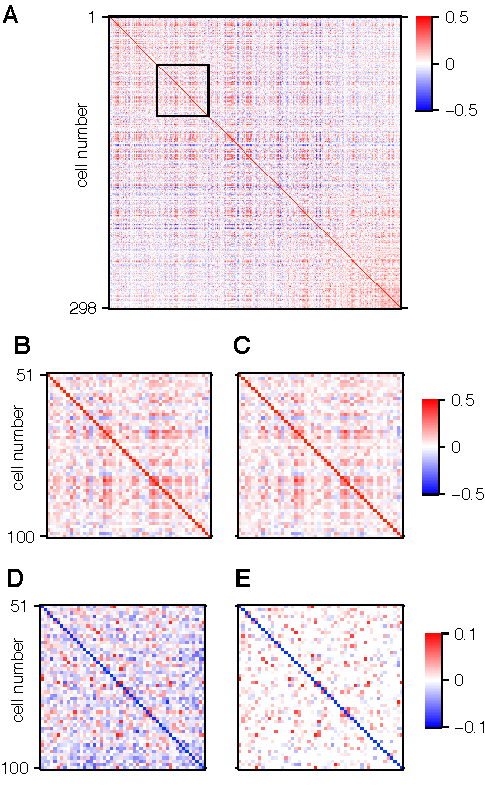
\includegraphics[width=8.3cm]{Figure01.pdf}
    \end{center}
    \caption{{\bf Illustration of regularized estimation of partial correlations.}
        {\bf A}. The sample correlation matrix of unprocessed somatic calcium signals from a population of cells in mouse visual cortex.
        The outlined square fragment is magnified in {\bf B}.
        {\bf C}. The same fragment of another estimate of the correlation matrix regularized to yield sparse partial correlations.
        Corresponding fragments of partial correlations matrices of the unregularized and regularized estimated are shown in {\bf D} and {\bf E}, respectively.
    }
    \label{fig:01}
\end{figure}

\begin{figure}[!ht]
    \begin{center}
        %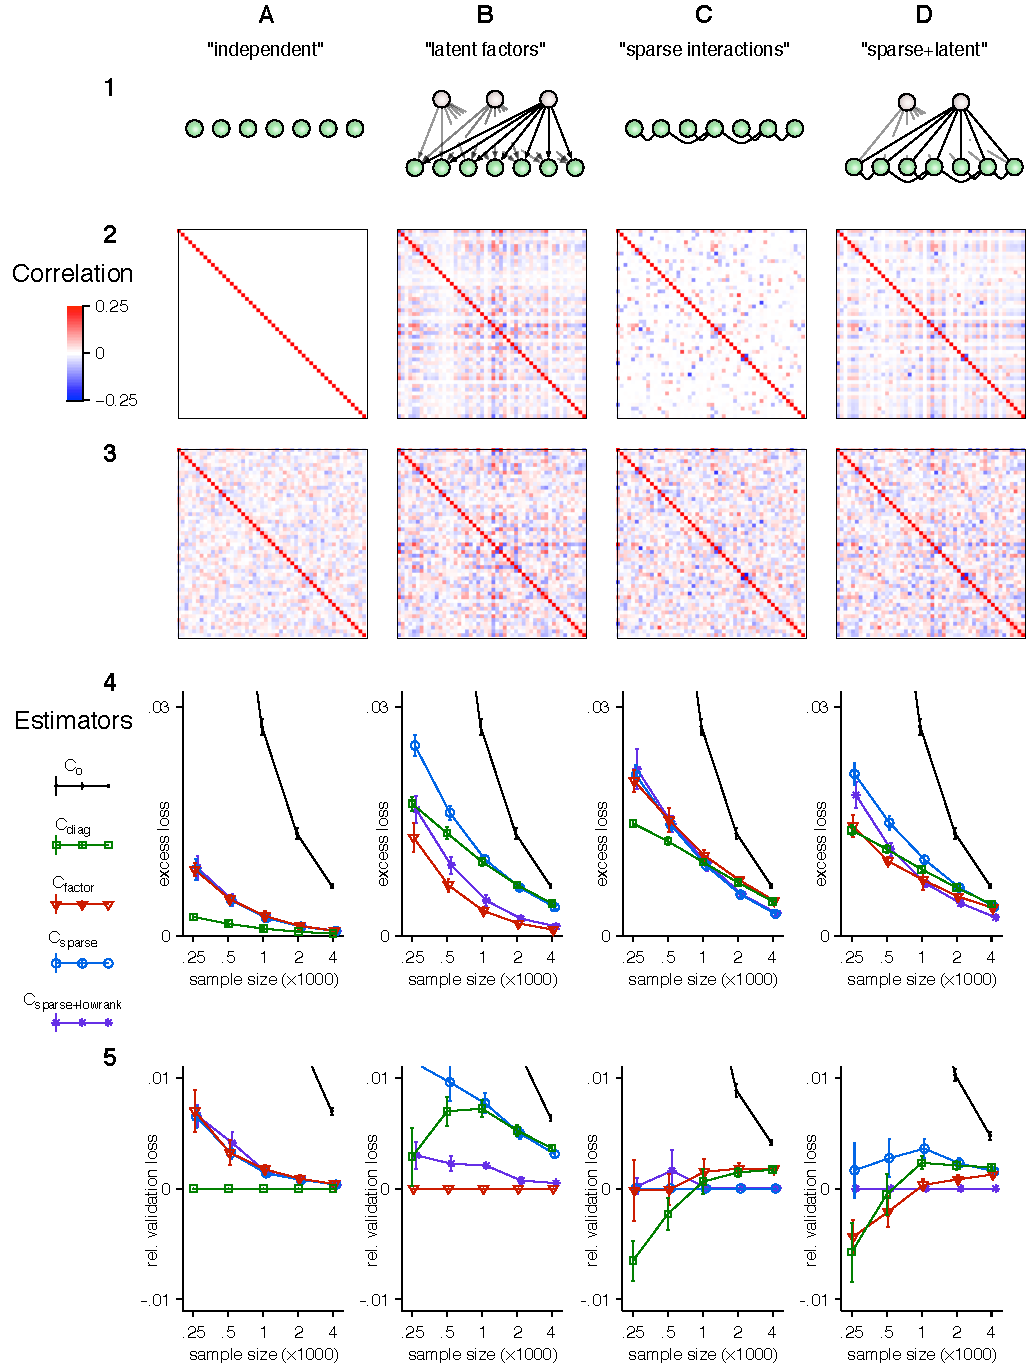
\includegraphics[width=17.35cm]{Figure02.pdf}
    \end{center}
    \caption{{\bf Estimators whose low-dimensional regularization targets can represent the structure of the true covariance matrix outperform other estimators.}
        {\bf Row 1.} Graphical representations of four types of low-dimensional structures of interactions between observed neurons (green spheres) and latent units (light-shaded spheres).
        In the \lq independent model\rq\;({\bf A}), observed neurons exert no linear effects on one another neither directly nor through interactions with common latent units. 
        In \lq latent factors\rq\;({\bf B}), the correlated activity of observed cells is driven by several latent units. 
        In \lq sparse interactions\rq\;({\bf C}), the correlation matrix is defined by a set of linear interactions between observed neurons. 
        In \lq sparse+latent\rq\;({\bf D}), correlations arise through direct linear interactions between some pairs of observed neurons and through interactions with common latent units. 
        {\bf Row 2.} Examples of $50\times 50$ correlation matrices corresponding to each type of low-dimensional structure. 
        The factor model ({\bf B}) has three latent units. 
        The partial correlation matrix of the sparse model ({\bf C}) is 73\% sparse.
        The \lq sparse+latent\rq\;matrix has one latent unit and its direct interactions are 78\% sparse.
        {\bf Row 3.} Examples of sample correlation matrices calculated from samples of 1000 observations taken from simulated random processes with corresponding correlation matrices from row 2.
        {\bf Row 4.} Average normalized Gaussian log-likelihood \emph{excess loss} (\ref{eq:excess-loss}) attained by each of the five estimators as a function of sample size. The error bars indicate the standard error of the mean based on 30 samples.
        {\bf Row 5.} Average normalized Gaussian log-likelihood \emph{validation loss} (\ref{eq:validation-loss}) attained by each of the five estimators. The values are relative to the validation loss of the estimator that matches the low-dimensional structure of the true covariance matrix. The error bars indicate the standard error of the mean based on 30 samples.
    }
    \label{fig:02}
\end{figure} 

\begin{figure}[!ht]
    \begin{center}
        %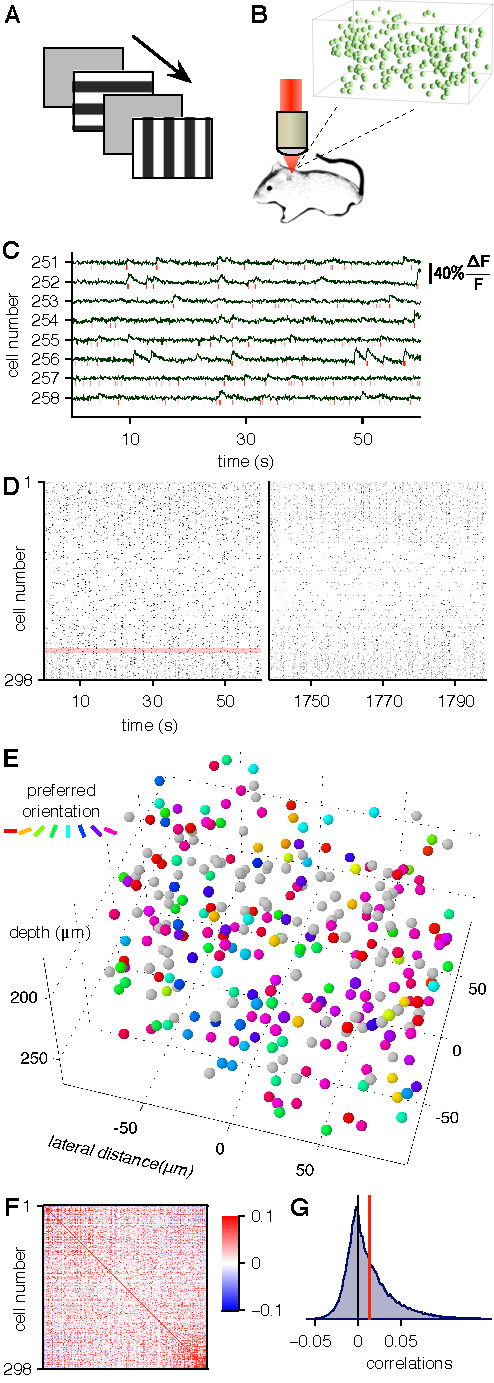
\includegraphics[width=8.3cm]{Figure03.pdf}
    \end{center}
    \caption{{\bf Acquisition of neural signals for the estimation of noise correlations.}
    Visual stimuli comprising full-field drifting gratings interleaved with blank screens ({\bf A}) were presented to anesthetized mice while two-photon recordings of somatic calcium signals were collected using fast 3D random-access microscopy ({\bf B}). The visual stimulus included an initial period with 16 directions of motion for orientation tuning followed by a longer (15--20 min) period of stimulation with only 2 or 5 directions of motion for the computation of the noise correlation matrix. 
    {\bf C.} Representative calcium signals from eight cells out of 298 cells downsampled to 20 Hz. The inferred firing rate binned in 150 ms intervals are indicated by red ticks below each trace.
    {\bf D.} The raster plot of the inferred firing rates, binned in 150 ms intervals, from the entire population from the first (left) and last (right) minute of the entire recording.  The traces from {\bf C} are highlighted in red.
    {\bf E.} The spatial arrangement and orientation tuning of the 298 cells from the imaged site.
    {\bf F.} The noise correlation matrix of the activity of the neural population. 
    {\bf G.} The histogram of the noise correlation coefficients with the mean indicated by the red line.
}
    \label{fig:03}
\end{figure}

\begin{figure}[!ht]
    \begin{center}
        %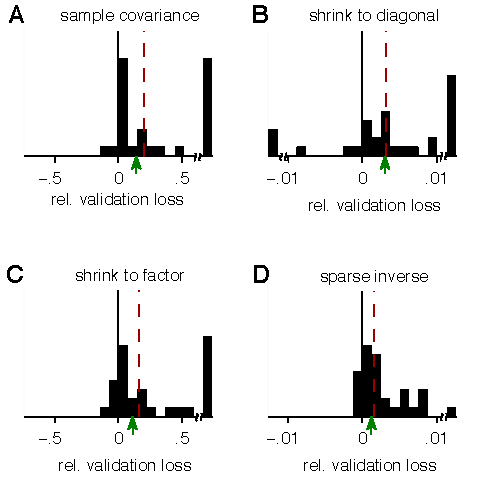
\includegraphics[width=8.3cm]{Figure04.pdf}
    \end{center}
    \caption{{\bf The sparse+lowrank estimator $C_{\sf sparse+lowrank}$ outperforms the other estimators on neural data.}
    {\bf A--D.} Histograms of average cross-validation loss differences of the respective estimators $C_0$, $C_{\sf diag}$, $C_{\sf factor}$, and $C_{\sf sparse}$ from $C_{\sf sparse+lowrank}$. 
    The histograms are based on 31 imaged sites in 24 mice. 
    All medians (red dashed lines) were significantly greater than zero, indicating the dominance of $C_{\sf sparse+lowrank}$ over the other estimators. 
    The green arrows indicate the results for the site shown in Fig.~\ref{fig:03} and Fig.~\ref{fig:05}
    }
    \label{fig:04}
\end{figure}
        
\begin{figure}[!ht]
    \begin{center}
        %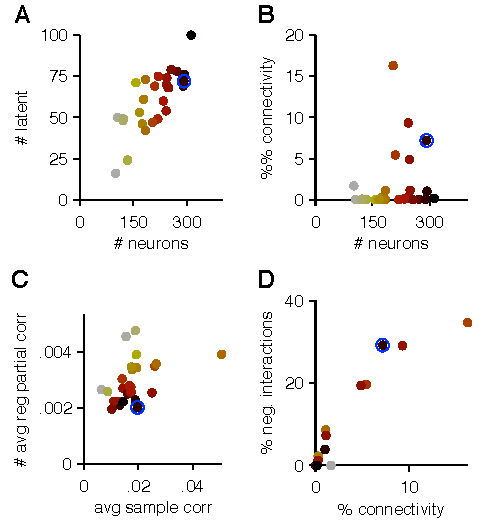
\includegraphics[width=17.35cm]{Figure05.pdf}
    \end{center}
    \caption{{\bf Example of low-dimensional correlation structure revealed by the sparse+low-rank estimator.}
    {\bf A.} The regularized estimate of the correlation matrix (top-right) closely approximates the sample correlation matrix (bottom left). 
    This close approximation is  also demonstrated by the scatter plot of the correlation coefficients produced by the two estimates ({\bf D}). 
    However, the partial correlation matrices from the two estimate show more pronounced differences ({\bf B} and {\bf E}). 
    {\bf C.} Furthermore, the partial correlation matrix of the regularized estimate is decomposed into a sparse component with 82.2\% off-diagonal zeros (bottom-left) and low-rank component of rank 15 (top-right).
    {\bf F.} The sparse component of the regularized partial correlation matrix had little resemblance to the sample correlations. The gray interval indicates the range of correlations containing 82.2\% of cells pairs, equal to the fraction of zeros in the sparse partial correlation matrix. This interval contained 58.9\% of the partial correlations. 
    {\bf G.} The graphical depiction of the positive (green) and negative (magenta) partial correlations as edges between observed neurons. The line density is proportional to the magnitude of the correlation.
    {\bf H.} A subset of neurons from the center of the cluster shown in {\bf G} showing the regularized partial correlations.
    {\bf I.} The same subset with sample correlations thresholded to match the sparsity of the regularized interactions.
}
\label{fig:05}
\end{figure}

\begin{figure}[!ht]
    \begin{center}
        %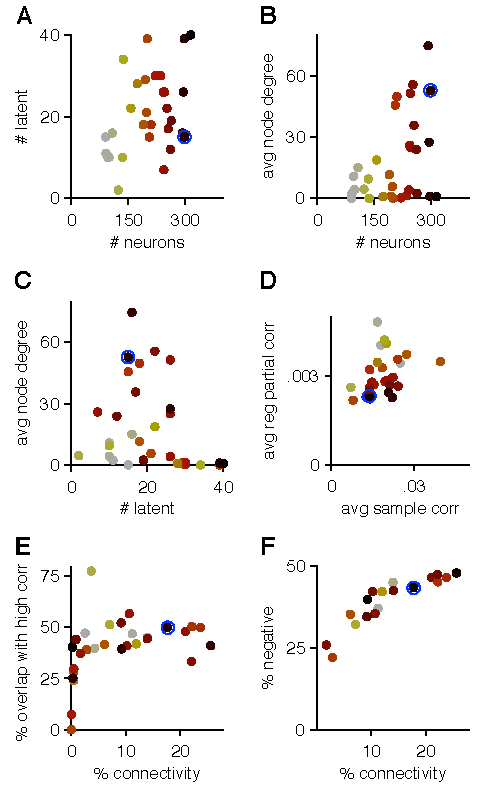
\includegraphics[width=17.35]{Figure06.pdf}
    \end{center}
    \caption{{\bf Properties of sparse+low-rank regularized estimates from all imaged sites}
    {\bf A.} The average sample correlations vs.~average partial correlations for each imaged site. In each plot, the red asterisk indicates the site shown in figures \ref{fig:03} and \ref{fig:05}.
    {\bf B.} The average node degree for sparse partial correlations vs.~population size in each imaged site. 
    {\bf C.} The number of inferred latent units vs.~population size in each imaged site.
    {\bf D.} The number latent units vs.~average node degree for sparse partial correlations for each site.
}
\label{fig:06}
\end{figure}

\begin{figure}[!ht]
    \begin{center}
        %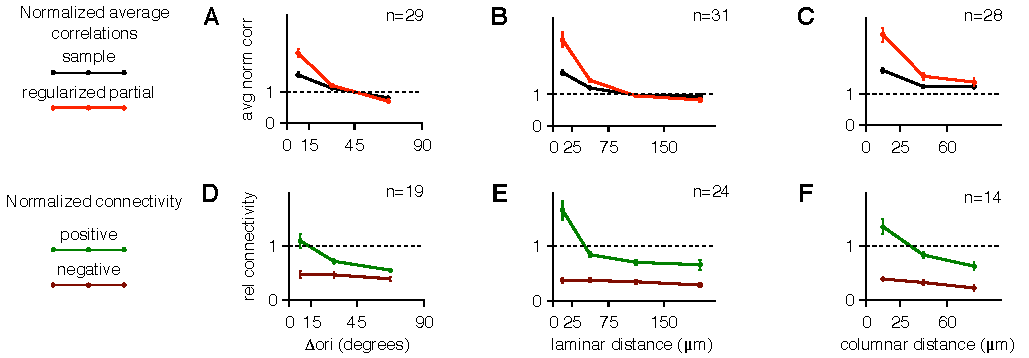
\includegraphics[width=17.35]{Figure07.pdf}
    \end{center}
    \caption{{\bf Dependence of correlations and partial correlations on orientation tuning differences and physical distance between cell pairs.}
    {\bf A--C.} Average sample correlations (black) and regularized partial correlations (red) between pairs of cells in the example site shown in previous figures. The correlations were normalized by the respective average correlations (\ref{fig:06}\;A).
    {\bf A.} Average correlations between pairs of neurons tuned to orientation with differences in preferred orientation in the intervals of 0--15$^\circ$, 15--45$^\circ$ and 45--90$^\circ$. 
    {\bf B.} Average correlations between pairs of neurons located at the same depth ($\pm$25$\mu$m) separated by lateral distances in the intervals of 0--25 $\mu$m, 25--75 $\mu$m, 75--150 $\mu$m, and 150+ $\mu$m.
    {\bf C.} Average correlations between pairs of neurons displaced laterally by less than 25 $\mu$m separated in depth by distances in the intervals of 0-25 $\mu$m, 25--60 $\mu$m, and 60+ $\mu$m.
    {\bf D--F.} Same measurements as {\bf A--D} averaged across multiple sites. Only sites that had at least 20 qualifying cell pairs in each of the intervals were included in the averages. The error bars indicate the standard error of the mean (often too small to be seen).
    {\bf G--I.} Normalized connectivity of positive (green) and negative (dark red) interactions from the sparse component of the regularized partial correlations in the example site show in previous figures. Normalized connectivity was computed as the fraction of pairs connected by interactions of corresponding signs in each interval divided by fraction of non-zero interactions across the entire site. The intervals are identical to those in {\bf A--C}.
    {\bf J--L.} Same measurements as in {\bf G--I} averaged across multiple sites. The error bars indicate the error of the mean. Only sites that had at least 20 qualifying pairs in each interval were included in the averages. 
}
\label{fig:07}
\end{figure}

\end{document}
